% ============================================================
%  Lucrare de Licență – Universitatea Politehnica Timișoara
%  Student: Iris-Daniela Dănilă
%  Aplicație: NutriLife
% ============================================================
\documentclass[12pt, a4paper, twoside]{report}

% ---------- pachete esențiale ----------
\usepackage{lmodern}
\usepackage[T1]{fontenc}
\usepackage[utf8]{inputenc}
\usepackage[romanian]{babel}

% ---------- caractere românești ----------
\DeclareUnicodeCharacter{0218}{\c{S}}
\DeclareUnicodeCharacter{0219}{\c{s}}
\DeclareUnicodeCharacter{021A}{\c{T}}
\DeclareUnicodeCharacter{021B}{\c{t}}
\usepackage{geometry}
\usepackage{graphicx}
\usepackage{amsmath, amssymb, amsfonts}
\usepackage{listings}
\usepackage{xcolor}
\usepackage{hyperref}
\usepackage{booktabs}
\usepackage{array}
\usepackage{tabularx}
\usepackage{longtable}
\usepackage{float}
\usepackage{caption}
\usepackage{subcaption}
\usepackage{wrapfig}
\usepackage{fancyhdr}
\usepackage{setspace}
\usepackage{titlesec}
\usepackage{enumitem}
\usepackage{microtype}
\usepackage{tocloft}
\usepackage{appendix}
\usepackage{indentfirst}
\usepackage{pdfpages}

% ---------- geometrie pagină ----------
\geometry{
  a4paper,
  top=2.5cm, bottom=2.5cm,
  left=3cm, right=2.5cm,
  headheight=2.5cm
}

% ---------- cale imagini ----------
\graphicspath{{images_iris/}{images_iris_white/}}

% ---------- spațiere ----------
\setstretch{1.15}

% ---------- evitarea spațiilor goale mari pe pagină ----------
% (implicit, clasa "report" folosește \flushbottom, care întinde spațiile
% elastice dintre paragrafe/liste/figuri pentru ca fiecare pagină să aibă
% exact aceeași înălțime; acest lucru produce goluri vizuale mari. Cu
% \raggedbottom paginile se termină la înălțimea naturală a conținutului.)
\raggedbottom

% ---------- spațiere mai compactă pentru liste ----------
\setlist[itemize]{topsep=4pt, itemsep=2pt, parsep=2pt}
\setlist[enumerate]{topsep=4pt, itemsep=2pt, parsep=2pt}

% ---------- spațiere mai compactă în jurul figurilor/tabelelor ----------
\setlength{\intextsep}{8pt plus 2pt minus 2pt}
\setlength{\textfloatsep}{10pt plus 2pt minus 2pt}
\setlength{\floatsep}{8pt plus 2pt minus 2pt}
\captionsetup{skip=6pt}

% ---------- culori cod ----------
\definecolor{codegreen}{rgb}{0,0.6,0}
\definecolor{codegray}{rgb}{0.5,0.5,0.5}
\definecolor{codepurple}{rgb}{0.58,0,0.82}
\definecolor{backcolour}{rgb}{0.97,0.97,0.97}
\definecolor{keywordblue}{rgb}{0.13,0.29,0.53}

\lstdefinestyle{mystyle}{
  backgroundcolor=\color{backcolour},
  commentstyle=\color{codegreen}\itshape,
  keywordstyle=\color{keywordblue}\bfseries,
  numberstyle=\tiny\color{codegray},
  stringstyle=\color{codepurple},
  basicstyle=\ttfamily\footnotesize,
  breakatwhitespace=false,
  breaklines=true,
  captionpos=b,
  keepspaces=true,
  numbers=left,
  numbersep=5pt,
  showspaces=false,
  showstringspaces=false,
  showtabs=false,
  tabsize=2,
  frame=single,
  rulecolor=\color{codegray}
}
\lstset{style=mystyle}

% ---------- stil pagini ----------
\pagestyle{fancy}
\fancyhf{}
\renewcommand{\chaptermark}[1]{\markboth{\thechapter.\ #1}{}}
\fancyhead[L]{\scriptsize\parbox[t]{0.65\headwidth}{%
  Universitatea Politehnica Timișoara \\
  Automatică și Calculatoare, 2026 \\
  Iris-Daniela Dănilă \\
  Aplicație Mobilă pentru Nutriție, Fitness și Bunăstare cu Inteligență Artificială On-Device}}
\fancyhead[R]{\raisebox{-1.4cm}{
\includegraphics[height=1.6cm]{upt_logo}}}
\fancyfoot[C]{\thepage}
\renewcommand{\headrulewidth}{0.4pt}

\fancypagestyle{plain}{%
  \fancyhf{}
  \fancyfoot[C]{\thepage}
  \renewcommand{\headrulewidth}{0pt}
}

% ---------- hyperref ----------
\hypersetup{
  colorlinks=true,
  linkcolor=blue!60!black,
  citecolor=green!50!black,
  urlcolor=blue!70!black,
  pdfauthor={Iris-Daniela Dănilă},
  pdftitle={Aplicație Mobilă pentru Nutriție, Fitness și Bunăstare cu Inteligență Artificială On-Device},
}

% ---------- font ----------
\renewcommand{\rmdefault}{phv}

% ---------- localizare tabele ----------
\AtBeginDocument{%
  \renewcommand{\tablename}{Tabelul}
}

% ---------- numerotare ecuații ----------
\numberwithin{equation}{section}

% ---------- titluri capitole ----------
\titleformat{\chapter}[display]
  {\normalfont\LARGE\bfseries}{\chaptertitlename\ \thechapter}{18pt}{\LARGE}
\titlespacing{\chapter}{0pt}{50pt}{30pt}

% ============================================================
\begin{document}

% ============================================================
%  PAGINA DE TITLU
% ============================================================
\begin{titlepage}
\thispagestyle{empty}

\noindent
\begin{minipage}[t]{0.60\textwidth}
  {\large\bfseries Automatică și Calculatoare}\\[0.3cm]
  {\large\bfseries 2026}
\end{minipage}%
\hfill
\begin{minipage}[t]{0.35\textwidth}
  \begin{flushright}
    
\includegraphics[width=\linewidth]{upt_logo}
  \end{flushright}
\end{minipage}

\vspace{5cm}
\begin{center}
  {\bfseries\LARGE Aplicație Mobilă pentru Nutriție,\\[0.5cm]
  Fitness și Bunăstare cu Inteligență\\[0.5cm]
  Artificială On-Device}
\end{center}

\vspace{4cm}

\noindent{\large\bfseries Candidat: Iris-Daniela Dănilă}\\[0.5cm]
\noindent{\large\bfseries Coordonator științific: As. Drd. Ing. Ionuț Grigore}

\vfill

\begin{center}
  {\large Sesiunea: Iulie 2026}
\end{center}
\setcounter{page}{1}
\end{titlepage}

% ============================================================
%  CUPRINS
% ============================================================
\tableofcontents
\newpage

% ============================================================
%  CAPITOLUL 1 – INTRODUCERE
% ============================================================
\chapter{Introducere}

\section{Motivație și context}

Obezitatea, sedentarismul și tulburările asociate unui stil de viață dezechilibrat
reprezintă unele dintre cele mai presante probleme de sănătate publică ale secolului XXI.
Potrivit Organizației Mondiale a Sănătății~\cite{who_obesity}, prevalența obezității la nivel global s-a
triplat din 1975, iar fenomenul afectează tot mai mult populația tânără. În paralel,
stresul cronic și absența unor tehnici accesibile de gestionare a emoțiilor contribuie la
deteriorarea stării de bine mentale. Aceste trei dimensiuni --- alimentația, mișcarea și
sănătatea mentală --- sunt profund interconectate, însă rareori sunt tratate împreună de
instrumentele digitale existente.

Aplicațiile mobile pentru monitorizarea sănătății au cunoscut o creștere accelerată în
ultimul deceniu. Cu toate acestea, majoritatea soluțiilor de pe piață prezintă cel puțin
una dintre limitările următoare:

\begin{enumerate}
  \item Funcționalitățile „inteligente'', precum recunoașterea alimentelor din fotografii,
    depind exclusiv de conexiunea la internet și de servere externe, către care sunt
    transmise imaginile utilizatorului;
  \item Lipsa unui asistent conversațional integrat, disponibil offline, care să ofere
    îndrumare personalizată;
  \item Absența unor mecanisme de gamificare suficient de bine proiectate pentru a susține
    motivația pe termen lung;
  \item Tratarea izolată a nutriției, activității fizice și sănătății mentale, fără o
    viziune holistică unificată;
  \item Modele de monetizare agresive, cu funcționalități de bază blocate în spatele unor
    abonamente costisitoare.
\end{enumerate}

\textbf{NutriLife} a fost concepută pentru a acoperi aceste lacune, construind un ecosistem
mobil coerent în care toate aspectele relevante ale unui stil de viață sănătos sunt
gestionate dintr-un singur loc. Trăsătura sa centrală este rularea modelelor de inteligență
artificială direct pe dispozitivul utilizatorului. Această alegere arhitecturală are trei
avantaje majore: \emph{confidențialitatea} (datele și fotografiile nu părăsesc niciodată
telefonul), \emph{disponibilitatea offline} (funcțiile inteligente operează fără semnal) și
\emph{costul zero de operare} (nu există servere de inferență de întreținut).

\section{Obiectivele lucrării}

Obiectivele principale ale acestei lucrări de licență sunt:

\begin{itemize}
  \item Proiectarea și implementarea unei aplicații mobile React Native complete, cu
    navigare pe mai multe ecrane, persistență locală a datelor și suport pentru temă
    vizuală clară/întunecată.
  \item Integrarea unui model ONNX de recunoaștere a alimentelor (\textit{EfficientNet-B0}
    antrenat pe Food-101), care rulează complet offline, direct pe dispozitiv.
  \item Integrarea unui model de limbaj cuantizat (\textit{SmolLM2-360M-Instruct}, q4) pentru
    asistentul virtual de nutriție, tot offline și on-device, incluzând implementarea unui
    tokenizator BPE pe nivel de octeți și a buclei de generare autoregresivă cu cache KV.
  \item Conectarea aplicației la surse de date publice de nutriție și rețete (USDA
    FoodData Central și TheMealDB).
  \item Construirea unui sistem de gamificare funcțional, cu XP, niveluri, ranguri, provocări
    zilnice și realizări, menit să crească angajamentul utilizatorului.
  \item Implementarea unor module native Android (contor de pași și notificări programate),
    fără dependențe terțe fragile.
  \item Demonstrarea viabilității inferenței locale a modelelor de rețele neuronale moderne
    pe dispozitive mobile cu resurse limitate.
\end{itemize}

\section{Structura lucrării}

Lucrarea este organizată în zece capitole:
\begin{itemize}
  \item \textbf{Capitolul 2} prezintă stadiul actual al domeniului, comparând aplicații
    similare existente cu NutriLife.
  \item \textbf{Capitolul 3} descrie tehnologiile și instrumentele utilizate.
  \item \textbf{Capitolul 4} prezintă arhitectura generală, structura proiectului, magazinul
    de stare și sistemul de navigare.
  \item \textbf{Capitolul 5} detaliază modelul de date și persistența cu Zustand și
    AsyncStorage, precum și formulele nutriționale.
  \item \textbf{Capitolul 6} descrie în detaliu modulele funcționale ale fiecărui ecran.
  \item \textbf{Capitolul 7} analizează integrarea celor două modele de inteligență
    artificială.
  \item \textbf{Capitolul 8} prezintă modulele native Android (pași și notificări).
  \item \textbf{Capitolul 9} tratează testarea și evaluarea aplicației.
  \item \textbf{Capitolul 10} descrie compilarea, configurarea și rularea aplicației, împreună
    cu provocările de mediu întâmpinate.
  \item \textbf{Capitolul 11} concluzionează lucrarea și propune direcții viitoare.
\end{itemize}

% ============================================================
%  CAPITOLUL 2 – STATE OF THE ART
% ============================================================
\chapter{Stadiul actual al domeniului}

Acest capitol analizează soluțiile existente pe piață, grupate pe categorii, și le compară
cu abordarea adoptată în NutriLife. Scopul nu este de a critica produse mature, ci de a
poziționa contribuția lucrării în raport cu acestea.

\section{Aplicații de monitorizare nutrițională}

\subsection{MyFitnessPal}

MyFitnessPal este probabil cea mai cunoscută aplicație de urmărire calorică la nivel global,
cu o bază de date ce depășește 14 milioane de alimente. Utilizatorul poate înregistra mese
prin scanarea codurilor de bare, prin căutare manuală sau prin import din rețete.

\textbf{Comparație cu NutriLife:} MyFitnessPal funcționează aproape exclusiv online și
blochează multe funcționalități avansate în spatele unui abonament premium. Nu include un
asistent conversațional local și nu oferă recunoaștere de alimente care să ruleze pe
dispozitiv. NutriLife adaugă recunoașterea AI a preparatelor din imagini, rulată complet
local, și un antrenor virtual disponibil offline, păstrând totuși accesul la o bază de date
nutrițională vastă prin API-ul USDA.

\subsection{Cronometer}

Cronometer se remarcă prin acuratețea datelor, urmărind nu doar macronutrienții, ci și
micronutrienții (vitamine, minerale). Este preferat de sportivi și de persoane cu regimuri
speciale.

\textbf{Comparație cu NutriLife:} Cronometer nu integrează inteligență artificială locală,
nu are gamificare și nu abordează sănătatea mentală. Este o unealtă puternică pentru
utilizatori avansați, dar poate fi intimidantă pentru publicul general. NutriLife vizează
accesibilitatea, combinând urmărirea nutrițională de bază cu instrumente de motivare și de
relaxare.

\subsection{Lose It!}

Lose It! oferă urmărire calorică, scanare de coduri de bare și un modul de exerciții.
Versiunea premium include recunoaștere de alimente din imagini printr-un serviciu cloud.

\textbf{Comparație cu NutriLife:} Recunoașterea din imagini în Lose It! depinde de un server
extern, ceea ce presupune conexiune la internet și transmiterea fotografiilor către terți.
NutriLife rulează modelul EfficientNet-B0 direct pe dispozitiv, fără a trimite date nicăieri
--- un avantaj clar de confidențialitate.

\section{Aplicații de fitness și activitate fizică}

\subsection{Google Fit și Apple Health}

Google Fit și Apple Health sunt platforme de referință pentru agregarea datelor de sănătate
pe Android, respectiv iOS. Colectează date de la senzori (pași, ritm cardiac, somn) și din
aplicații terțe, oferind un tablou de bord general.

\textbf{Comparație cu NutriLife:} Acestea sunt ecosisteme de agregare a datelor, nu produse
centrate pe utilizator. Nu includ un asistent conversațional, nu au gamificare și nu
abordează nutriția sau meditația în mod integrat. NutriLife adoptă o abordare diferită: un
singur produs care acoperă toate dimensiunile relevante și care, în plus, își numără proprii
pași printr-un modul nativ.

\subsection{Strava}

Strava este centrată pe activitățile sportive (alergare, ciclism, înot), cu funcții sociale
puternice (segmente, clasamente, feed de activitate).

\textbf{Comparație cu NutriLife:} Strava nu urmărește nutriția, nu are meditație și nu
integrează AI local. NutriLife nu concurează cu Strava pe zona de performanță sportivă, ci
se adresează utilizatorilor care doresc să-și îmbunătățească stilul de viață general.

\section{Aplicații de meditație și sănătate mentală}

\subsection{Headspace și Calm}

Headspace și Calm sunt cele mai cunoscute aplicații de meditație ghidată, cu sute de sesiuni
structurate tematic și conținut premium (voci profesionale, povești pentru somn, muzică de
relaxare).

\textbf{Comparație cu NutriLife:} Ambele sunt produse premium dedicate exclusiv meditației.
NutriLife include un modul de respirație ghidată (cu tehnici precum \textit{box breathing}
sau 4-7-8), animat și temporizat, ca parte a unui ecosistem mai larg, fără a pretinde a
înlocui o aplicație specializată, dar oferind un punct de intrare gratuit în practica
mindfulness, recompensat prin sistemul de gamificare.

\section{Aplicații cu asistent AI pentru nutriție}

\subsection{Noom}

Noom combină urmărirea calorică cu coaching uman și psihologie comportamentală: utilizatorii
sunt asignați unui coach real, în cadrul unui program structurat și costisitor.

\textbf{Comparație cu NutriLife:} Modelul Noom implică oameni reali și un abonament scump.
NutriLife democratizează accesul la îndrumare prin intermediul unui model de limbaj rulat
local, care oferă răspunsuri instant și gratuit, fără a înlocui un nutriționist profesionist
și fără a transmite date personale.

\section{Rezumat comparativ}

Tabelul~\ref{tab:comparatie} sintetizează funcționalitățile principale ale aplicațiilor
analizate față de NutriLife.

\begin{table}[H]
\centering
\caption{Comparație între NutriLife și aplicații similare}
\label{tab:comparatie}
\footnotesize
\setlength{\tabcolsep}{4pt}
\begin{tabularx}{\textwidth}{>{\raggedright\arraybackslash}p{3.1cm}*{5}{>{\centering\arraybackslash}X}}
\toprule
\textbf{Funcțio\-nalitate} & \textbf{Nutri\-Life} & \textbf{MyFit\-nessPal} & \textbf{Head\-space} & \textbf{Strava} & \textbf{Noom} \\
\midrule
Urmărire nutriție & Da & Da & Nu & Nu & Da \\
Recunoaștere AI offline & Da & Nu & Nu & Nu & Nu \\
Asistent AI local & Da & Nu & Nu & Nu & Nu \\
Meditație & Da & Nu & Da & Nu & Nu \\
Gamificare & Da & Parțial & Nu & Parțial & Nu \\
Monitorizare pași & Da & Da & Nu & Da & Nu \\
Rețete integrate & Da & Nu & Nu & Nu & Nu \\
Funcționare offline & Da & Limitată & Limitată & Nu & Nu \\
\bottomrule
\end{tabularx}
\end{table}

Tabelul arată că NutriLife este singura aplicație din comparație care combină toate aceste
dimensiuni simultan, cu un accent deosebit pe funcționarea offline prin modele AI locale și
pe protecția confidențialității.

% ============================================================
%  CAPITOLUL 3 – TEHNOLOGII ȘI INSTRUMENTE
% ============================================================
\chapter{Tehnologii și instrumente utilizate}

\section{React Native}

React Native este un framework open-source dezvoltat de Meta care permite construirea de
aplicații mobile native pentru iOS și Android dintr-o singură bază de cod
JavaScript/TypeScript~\cite{reactnative}. Spre deosebire de soluțiile de tip \textit{WebView}, componentele
React Native se traduc în elemente de interfață native, rezultând o performanță și o
experiență de utilizare apropiate de aplicațiile native scrise manual.

NutriLife utilizează React Native în varianta \textbf{„bare''} (versiunea 0.74.5), fără
Expo. Această alegere a fost obligatorie: integrarea ONNX Runtime și a modulelor native
proprii (senzorul de pași, notificările) necesită acces complet la stratul nativ Android și
la mecanismul de \textit{autolinking}, lucru pe care fluxul gestionat de Expo nu îl permite
fără ejectare. Motorul JavaScript este Hermes~\cite{hermes}, activat implicit, optimizat pentru pornire
rapidă și consum redus de memorie.

\section{TypeScript}

TypeScript~\cite{typescript} este un superset al JavaScript care adaugă tipare statice. Într-o aplicație cu
multiple structuri de date interdependente --- profil de utilizator, intrări de jurnal,
ținte nutriționale, stare de gamificare, mesaje de chat, răspunsuri ale modelelor ---
tiparea statică reduce semnificativ riscul erorilor la rulare și ușurează refactorizarea.
Toate fișierele sursă ale proiectului folosesc extensiile \texttt{.ts} sau \texttt{.tsx},
iar interfețele de domeniu sunt centralizate în \texttt{src/\allowbreak store/\allowbreak types.ts}.

\section{React Navigation}

Navigarea este implementată cu React Navigation (v6)~\cite{reactnav}, folosind o combinație de două
tipuri de navigatoare:
\begin{itemize}
  \item un \texttt{NativeStackNavigator} rădăcină, care gestionează poarta de
    \textit{onboarding} și ecranele deschise „peste'' tab-uri (căutare, detalii aliment,
    rețete, calendar, setări etc.);
  \item un \texttt{BottomTabNavigator} cu cinci tab-uri principale, cu un buton central
    proeminent pentru scanare.
\end{itemize}
Culorile, înălțimea și iconițele barei de navigare sunt derivate dinamic din tema activă.

\section{Zustand și AsyncStorage}

Spre deosebire de soluțiile care țin starea exclusiv local în fiecare ecran, NutriLife
folosește un \textbf{magazin de stare global} construit cu \textbf{Zustand}~\cite{zustand} --- o bibliotecă
minimalistă, fără \textit{boilerplate}-ul Redux. Întregul magazin este învelit în
\textit{middleware}-ul \texttt{persist}, configurat cu un adaptor către
\texttt{@react-native-async-storage/\allowbreak async-storage}~\cite{asyncstorage}. Astfel, orice modificare a stării
(adăugarea unei mese, băutul unui pahar de apă, completarea unei provocări) este serializată
automat JSON și salvată pe dispozitiv, fiind rehidratată la următoarea pornire. AsyncStorage
funcționează ca un magazin asincron de perechi cheie-valoare.

\section{ONNX Runtime React Native}

ONNX (Open Neural Network Exchange)~\cite{onnxformat} este un format deschis pentru reprezentarea modelelor de
\textit{machine learning}. ONNX Runtime este motorul de inferență transversal dezvoltat de
Microsoft, optimizat pentru eficiență pe resurse limitate~\cite{onnxruntime}.

\texttt{onnxruntime-react-native} (versiunea 1.20.0)~\cite{onnxrn} este legătura nativă care expune ONNX
Runtime în React Native. NutriLife utilizează această bibliotecă pentru ambele modele:
EfficientNet-B0 pentru clasificarea alimentelor și SmolLM2-360M pentru asistentul de chat.
Inferența se realizează complet pe dispozitiv. Alegerea versiunii 1.20.0 nu a fost
arbitrară: ea este versiunea minimă care recunoaște atributul \texttt{softcap} al
operatorului contributiv \texttt{GroupQueryAttention}, prezent în graful modelului de limbaj
(detaliile sunt discutate în Capitolul~7).

\section{EfficientNet-B0 și setul de date Food-101}

EfficientNet-B0 este cea mai mică variantă din familia EfficientNet propusă de Google~\cite{efficientnet}, care
folosește o scalare compusă echilibrată a adâncimii, lățimii și rezoluției rețelei.
Modelul folosit în NutriLife a fost antrenat pe setul de date \textbf{Food-101}~\cite{food101}, care conține
101.000 de imagini distribuite uniform între 101 clase de preparate culinare, și este
exportat în format ONNX (intrare \texttt{[1,3,224,224]}, ieșire \texttt{[1,101]}).

\section{SmolLM2-360M-Instruct}

SmolLM2-360M-Instruct, dezvoltat de Hugging Face~\cite{smollm2}, este un model de limbaj de mici dimensiuni
(360 de milioane de parametri) din familia de arhitecturi Llama, ajustat pentru urmărirea
instrucțiunilor. Pentru a rula pe telefon, NutriLife folosește varianta cuantizată la 4 biți
(\texttt{model\_q4.onnx}), cu activări și cache KV în \texttt{float32}. Modelul utilizează
\textit{Grouped-Query Attention} (5 capete de tip cheie/valoare, dimensiune cap 64) pe 32 de
straturi, cu un vocabular de 49.152 de jetoane.

\section{API-ul USDA FoodData Central}

USDA FoodData Central (\url{https://fdc.nal.usda.gov/}) este o bază de date publică,
guvernamentală, cu informații nutriționale pentru sute de mii de alimente~\cite{usda}. NutriLife
interoghează punctul terminal de căutare și normalizează rezultatele la valori „per 100 g''
(calorii, proteine, glucide, lipide), care apoi sunt scalate la cantitatea consumată de
utilizator.

\section{API-ul TheMealDB}

TheMealDB (\url{https://www.themealdb.com/api.php}) este un API public și gratuit cu mii de
rețete organizate pe categorii și zone geografice~\cite{themealdb}. NutriLife folosește punctele terminale de
căutare după denumire, filtrare pe categorii și obținerea detaliilor complete ale unui
preparat (ingrediente, cantități, instrucțiuni, link YouTube).

\section{Biblioteci de interfață și utilitare}

Tabelul~\ref{tab:pachete} listează celelalte dependențe importante ale proiectului.

\begin{table}[H]
\centering
\caption{Pachete suplimentare utilizate în NutriLife}
\label{tab:pachete}
\begin{tabularx}{\textwidth}{lX}
\toprule
\textbf{Pachet} & \textbf{Rol} \\
\midrule
\texttt{react-native-image-picker} & Captură foto sau selecție din galerie pentru scaner \\
\texttt{react-native-fs} & Copierea modelelor din \textit{assets} în directorul de documente \\
\texttt{react-native-svg} & Inele de progres, grafice cu bare/linii, paharul de apă \\
\texttt{react-native-linear-gradient} & Gradientele cardurilor, butoanelor și emblemelor \\
\texttt{react-native-vector-icons} & Setul de pictograme MaterialCommunityIcons \\
\texttt{jpeg-js} & Decodarea JPEG în date pixel brute (RGBA) pentru preprocesare \\
\texttt{react-native-safe-area-context} & Gestionarea zonelor de siguranță (notch, bară de stare) \\
\texttt{react-native-screens} & Optimizarea navigării prin componente native de ecran \\
\texttt{react-native-gesture-handler} & Gesturi native, necesar React Navigation \\
\bottomrule
\end{tabularx}
\end{table}

% ============================================================
%  CAPITOLUL 4 – ARHITECTURA APLICAȚIEI
% ============================================================
\chapter{Arhitectura aplicației}

\section{Prezentare generală}

NutriLife este structurată pe un model în trei straturi:
\begin{itemize}
  \item \textbf{Stratul de prezentare} --- ecranele (\texttt{screens}), componentele
    reutilizabile (\texttt{components}) și navigarea, responsabile cu interfața;
  \item \textbf{Stratul de servicii și stare} --- magazinul Zustand, serviciile de domeniu
    (nutriție, USDA, TheMealDB, antrenor, gamificare) și inferența modelelor;
  \item \textbf{Stratul de infrastructură} --- utilitarele de preprocesare a imaginilor,
    tokenizatorul BPE, managerul de sesiuni ONNX și modulele native Android.
\end{itemize}

Spre deosebire de o arhitectură în care fiecare ecran își gestionează izolat starea,
NutriLife centralizează datele într-un singur magazin Zustand persistat. Această decizie
simplifică sincronizarea între ecrane (de exemplu, adăugarea unei mese în jurnal
actualizează instantaneu inelul caloric din tabloul de bord, progresul provocărilor și
calendarul obiectivelor) și elimină duplicarea logicii de persistență.

\clearpage
\section{Cazurile de utilizare}

\begin{wrapfigure}[20]{r}{0.35\textwidth}
  \centering
  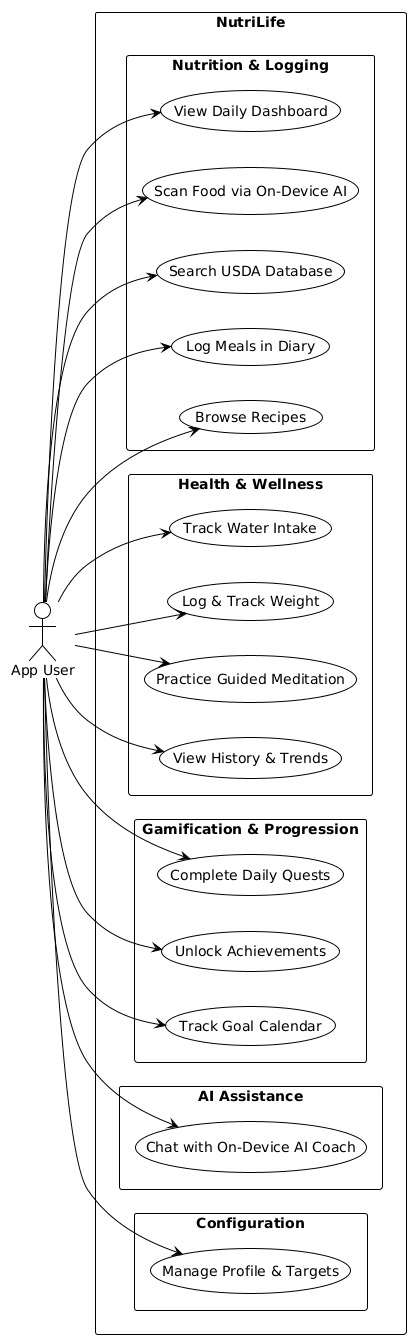
\includegraphics[width=0.33\textwidth, height=7cm, keepaspectratio]{diagrama_uml}
  \caption{Diagrama cazurilor de utilizare a aplicației NutriLife}
  \label{fig:usecase}
\end{wrapfigure}

Deoarece NutriLife nu are conturi de utilizator sau roluri multiple, diagrama cazurilor de
utilizare alăturată consideră un singur actor, \textbf{Utilizatorul}, care interacționează
direct cu toate funcționalitățile aplicației. Principalele cazuri de utilizare surprinse sunt
gestionarea jurnalului alimentar (fie prin căutare în USDA, fie prin scanarea AI a
preparatelor), consultarea antrenorului virtual conversațional, urmărirea hidratării, a
greutății și a sesiunilor de meditație, precum și interacțiunea cu sistemul de gamificare
(provocări zilnice, realizări și calendarul obiectivelor).

Cazurile de „scanare a alimentelor'' și „căutare în USDA'' sunt tratate ca alternative ale
aceluiași obiectiv --- adăugarea unei intrări în jurnal --- prima bazându-se pe inferența
locală a modelului EfficientNet-B0, iar a doua pe interogarea directă a bazei de date USDA.
În mod similar, actualizarea automată a progresului provocărilor zilnice și a nivelului de
experiență este declanșată indirect de aproape orice altă acțiune a utilizatorului (masă
înregistrată, apă băută, sesiune de meditație finalizată etc.), motiv pentru care aceste
relații sunt reprezentate în diagramă prin dependențe de tip \textit{extend}.

\section{Structura directorului de proiect}

\begin{lstlisting}[language=bash, caption={Structura simplificată a proiectului NutriLife}]
nutri-life2.0/
|-- android/                 # Proiectul nativ Android (Kotlin, Gradle)
|   `-- app/src/main/
|       |-- assets/models/   # Modelele ONNX + tokenizer (bundle in APK)
|       `-- java/com/nutrilife/  # Module native: StepCounter, Reminder
|-- models/                  # Modelele sursa (.onnx)
|-- scripts/                 # copy-models.js, fetch-tokenizer.js, dev-android.bat
|-- src/
|   |-- theme/               # colors.ts, ThemeContext.tsx, typography.ts
|   |-- store/               # useAppStore.ts (Zustand), types.ts
|   |-- services/
|   |   |-- usda.ts          # Client USDA FoodData Central
|   |   |-- mealdb.ts        # Client TheMealDB
|   |   |-- nutrition.ts     # BMR / TDEE / macronutrienti / IMC
|   |   |-- coach.ts         # Orchestrarea asistentului + fallback
|   |   |-- levels.ts        # Curba XP si rangurile
|   |   |-- challenges.ts    # Provocarile zilnice
|   |   |-- achievements.ts  # Realizarile pe niveluri
|   |   |-- steps.ts         # Punte JS pentru contorul de pasi
|   |   |-- notifications.ts # Punte JS pentru notificari
|   |   `-- onnx/            # modelManager, foodModel, imagePreprocess,
|   |                        # food101Labels, tokenizer, llm
|   |-- hooks/               # useNutrition, useGamification, useSteps
|   |-- components/          # Screen, Card, Button, ProgressRing, Charts...
|   |-- screens/             # Cele ~16 ecrane ale aplicatiei
|   `-- navigation/          # RootNavigator, TabNavigator, types
|-- App.tsx                  # Componenta radacina (provideri + onboarding gate)
`-- index.js                 # Punctul de intrare
\end{lstlisting}

\section{Magazinul de stare (Zustand)}

Fișierul \texttt{src/\allowbreak store/\allowbreak useAppStore.ts} definește un singur \textit{hook} de stare,
\texttt{useAppStore}, care expune atât datele cât și acțiunile de mutație. Magazinul este
învelit în \texttt{persist} și folosește un \texttt{partialize} explicit pentru a alege ce
felii se salvează pe disc (profil, jurnal, hidratare, greutăți, meditații, antrenamente,
chat, gamificare, pași). Un \textit{flag} \texttt{hydrated} semnalează momentul în care
datele persistate au fost reîncărcate, astfel încât interfața să afișeze un indicator de
încărcare până atunci.

\section{Sistemul de navigare}

\begin{table}[H]
\centering
\caption{Tab-urile barei de navigare principale}
\label{tab:navigare}
\begin{tabularx}{\textwidth}{llX}
\toprule
\textbf{Tab} & \textbf{Etichetă} & \textbf{Ecran} \\
\midrule
Home & Acasă & Tabloul de bord zilnic (calorii, macro, apă, pași, provocări) \\
Diary & Jurnal & Jurnalul alimentar pe mese, cu navigare pe zile \\
Scan & Scanare & Buton central proeminent: recunoașterea AI a alimentelor \\
Coach & Antrenor & Asistentul virtual de nutriție (SmolLM2) \\
More & Mai mult & Hub către celelalte module (rețete, calendar, meditație etc.) \\
\bottomrule
\end{tabularx}
\end{table}

Ecranele secundare (\texttt{FoodSearch}, \texttt{FoodDetail}, \texttt{Water},
\texttt{Meditation}, \texttt{History}, \texttt{Weight}, \texttt{Settings},
\texttt{Achievements}, \texttt{Challenges}, \texttt{Recipes}, \texttt{RecipeDetail},
\texttt{GoalCalendar}) sunt înregistrate în navigatorul de tip stivă rădăcină și sunt
deschise fie din tab-uri, fie din ecranul „Mai mult''.

\section{Inițializarea și onboarding-ul}

Componenta rădăcină \texttt{App.tsx} încapsulează aplicația în furnizorii necesari
(\texttt{GestureHandlerRootView}, \texttt{SafeAreaProvider}, \texttt{ThemeProvider}) și
într-un \texttt{NavigationContainer} a cărui temă este sincronizată cu tema aplicației. La
prima lansare, în absența unui profil completat, navigatorul rădăcină afișează ecranul de
\textit{onboarding}, în care utilizatorul introduce: numele, sexul, vârsta, înălțimea,
greutatea, nivelul de activitate și obiectivul (slăbire/menținere/creștere). Pe baza acestor
date se calculează automat țintele zilnice (calorii, macronutrienți, apă), iar profilul este
salvat în magazin. La lansările ulterioare, aplicația deschide direct tabloul de bord.

\section{Tema vizuală și suportul pentru modul întunecat}

\texttt{src/\allowbreak theme/\allowbreak colors.ts} definește două palete complete --- \texttt{lightTheme} și
\texttt{darkTheme} --- care împărtășesc aceeași formă (aceleași chei), astfel încât
componentele să poată consuma exclusiv obiectul de temă, fără culori codate fix.
\texttt{ThemeContext} rezolvă tema activă în funcție de preferința utilizatorului
(clar/întunecat/sistem) și de schema de culoare a sistemului de operare. Comutarea temei se
face dintr-un singur buton din tabloul de bord sau din ecranul de setări.

\begin{table}[H]
\centering
\caption{Câteva culori-cheie ale celor două teme}
\label{tab:teme}
\begin{tabularx}{\textwidth}{lXX}
\toprule
\textbf{Rol} & \textbf{Temă clară} & \textbf{Temă întunecată} \\
\midrule
Fundal aplicație & \#F5F7F6 & \#0C100E \\
Card / suprafață & \#FFFFFF & \#161C19 \\
Culoare primară (verde) & \#16A571 & \#23D196 \\
Accent & \#FF7A59 & \#FF8C6B \\
Text principal & \#11201B & \#ECF2EF \\
Apă & \#3AB7E8 & \#4FC3F7 \\
\bottomrule
\end{tabularx}
\end{table}

\section{Proiectarea interfeței și biblioteca de componente}

Interfața NutriLife urmează un limbaj vizual unitar și modern: carduri cu colțuri rotunjite,
gradiente discrete pe elementele de accent (butoane, embleme de nivel, paharul de apă),
spațiere consistentă pe o grilă de $4$~pt și o ierarhie tipografică clară. Pentru a asigura
coerența și a evita culorile codate fix, toate ecranele consumă culorile exclusiv din obiectul
de temă (Secțiunea precedentă), iar elementele comune sunt extrase într-o \textbf{bibliotecă de
componente reutilizabile} (\texttt{src/\allowbreak components/}), prezentată în Tabelul~\ref{tab:componente}.

\begin{table}[H]
\centering
\caption{Componente reutilizabile principale}
\label{tab:componente}
\begin{tabularx}{\textwidth}{lX}
\toprule
\textbf{Componentă} & \textbf{Rol} \\
\midrule
\texttt{Screen} & Container de pagină cu zone de siguranță, fundal tematic și scroll opțional \\
\texttt{Card} & Suprafață elevată reutilizabilă, cu variantă „plată'' pentru fundaluri colorate \\
\texttt{Button} & Buton cu gradient, variante (primar/secundar/fantomă) și stare de încărcare \\
\texttt{ProgressRing} & Inel de progres circular (SVG) pentru bilanțul caloric \\
\texttt{MacroBar} & Bare de progres pentru macronutrienți \\
\texttt{Charts} & Grafice cu bare și linii (SVG) pentru istoric și greutate \\
\texttt{WaterGlass} & Pahar stilizat care se umple proporțional (SVG) \\
\texttt{LevelBadge} & Emblemă hexagonală de rang (SVG) \\
\texttt{Chip}, \texttt{SegmentedControl} & Selectoare compacte și filtre \\
\bottomrule
\end{tabularx}
\end{table}

Vizualizările de date (inelele de progres, graficele, paharul de apă, emblema hexagonală de
rang) sunt desenate vectorial cu \texttt{react-native-svg}, fiind astfel scalabile și
independente de densitatea ecranului, iar pictogramele provin din setul MaterialCommunityIcons.
Un element de UX distinctiv este butonul central proeminent de scanare din bara de navigare,
ridicat deasupra celorlalte tab-uri pentru a evidenția funcția-cheie a aplicației. Comutarea
între tema clară și cea întunecată se reflectă instantaneu în toate ecranele, fără repornire.

\section{Utilizarea instrumentelor de inteligență artificială în dezvoltare}

Pe parcursul dezvoltării codului sursă au fost folosite, punctual, instrumente de
inteligență artificială generativă, exclusiv ca ajutor auxiliar:

\begin{itemize}
  \item generarea unor fragmente de cod repetitiv (de exemplu componente de interfață
    asemănătoare sau cod de tip \textit{boilerplate});
  \item asistență la depanare, prin explicarea unor mesaje de eroare întâlnite la
    compilarea proiectului Android sau la exportul modelelor ONNX;
  \item sugerarea unor nume de variabile/funcții și a unor comentarii de cod pentru
    porțiuni de cod scrise de mine, în scopul îmbunătățirii lizibilității.
\end{itemize}

Arhitectura, deciziile tehnice și implementarea efectivă îmi aparțin în întregime;
sugestiile primite au fost verificate și adaptate manual înainte de a fi integrate în
proiect.

% ============================================================
%  CAPITOLUL 5 – GESTIUNEA DATELOR ȘI PERSISTENȚA
% ============================================================
\chapter{Gestiunea datelor și persistența}

\section{Modelul de date}

NutriLife definește un set de interfețe TypeScript care modelează entitățile principale,
centralizate în \texttt{src/\allowbreak store/\allowbreak types.ts}. Datele zilnice sunt organizate pe chei de tip
dată calendaristică (\texttt{YYYY-MM-DD}), ceea ce permite accesul eficient la orice zi.

\subsection{Profilul utilizatorului și țintele}

\begin{lstlisting}[language=JavaScript, caption={Profilul și țintele nutriționale}]
export interface Profile {
  name: string;
  sex: 'male' | 'female';
  age: number;
  heightCm: number;
  weightKg: number;
  activity: 'sedentary' | 'light' | 'moderate' | 'active' | 'veryActive';
  goal: 'lose' | 'maintain' | 'gain';
  calorieTargetOverride?: number | null;
}

export interface NutritionTargets {
  calories: number;
  carbs: number;   // grame
  protein: number; // grame
  fat: number;     // grame
  waterMl: number;
}
\end{lstlisting}

\subsection{Jurnalul alimentar}

\begin{lstlisting}[language=JavaScript, caption={Intrarea de jurnal și jurnalul zilnic}]
export interface FoodEntry {
  id: string;
  name: string;
  meal: 'breakfast' | 'lunch' | 'dinner' | 'snack';
  loggedAt: string;
  amount: number;
  unit: string;
  calories: number;
  carbs: number;
  protein: number;
  fat: number;
  source: 'usda' | 'ai-scan' | 'manual';
  fdcId?: number;
  confidence?: number; // 0..1, daca provine din scaner
}

export type Diary = Record<string, FoodEntry[]>; // cheie = YYYY-MM-DD
export type WaterLog = Record<string, number>;   // ml pe zi
\end{lstlisting}

Pe lângă acestea, modelul mai cuprinde: \texttt{WeightEntry} (greutate per zi),
\texttt{MeditationSession} (preset, durată, moment), \texttt{WorkoutEntry} (tip de
antrenament, durată), \texttt{ChatMessage} (rol, conținut, stare de generare) și
structurile de gamificare (XP, provocări revendicate, provocări manuale completate,
realizări revendicate).

\section{Persistența cu Zustand și AsyncStorage}

Magazinul aplică un \texttt{partialize} explicit pentru a persista doar feliile relevante,
excluzând câmpurile tranzitorii precum \texttt{hydrated}. Listing-ul~\ref{lst:persist}
arată configurarea \textit{middleware}-ului.

\begin{lstlisting}[language=JavaScript, caption={Configurarea persistenței}, label={lst:persist}]
export const useAppStore = create<AppState>()(
  persist(
    (set, get) => ({ /* stare + actiuni */ }),
    {
      name: 'nutrilife-store-v1',
      storage: createJSONStorage(() => AsyncStorage),
      partialize: state => ({
        onboarded: state.onboarded,
        profile: state.profile,
        diary: state.diary,
        water: state.water,
        weights: state.weights,
        meditations: state.meditations,
        workouts: state.workouts,
        chat: state.chat,
        steps: state.steps,
        xp: state.xp,
        /* ... restul feliilor de gamificare ... */
      }),
      onRehydrateStorage: () => state => state?.setHydrated(true),
    },
  ),
);
\end{lstlisting}

\section{Formulele nutriționale}

Țintele zilnice sunt calculate în \texttt{src/\allowbreak services/\allowbreak nutrition.ts}. Metabolismul bazal
(BMR) se estimează cu ecuația Mifflin--St Jeor~\cite{mifflin}:

\begin{equation}
\text{BMR} = 10\,w + 6{,}25\,h - 5\,a +
\begin{cases} +5 & \text{bărbați} \\ -161 & \text{femei} \end{cases}
\end{equation}

unde $w$ este greutatea (kg), $h$ înălțimea (cm) și $a$ vârsta (ani). Necesarul caloric
total (TDEE) se obține înmulțind BMR cu un factor de activitate
(Tabelul~\ref{tab:activitate}):

\begin{equation}
\text{TDEE} = \text{BMR} \times f_{\text{activitate}}
\end{equation}

\begin{table}[H]
\centering
\caption{Factorii de activitate fizică}
\label{tab:activitate}
\begin{tabularx}{\textwidth}{lXl}
\toprule
\textbf{Nivel} & \textbf{Descriere} & \textbf{Factor} \\
\midrule
Sedentar & Puțină sau deloc mișcare & 1{,}20 \\
Ușor & 1--3 zile/săptămână & 1{,}375 \\
Moderat & 3--5 zile/săptămână & 1{,}55 \\
Activ & 6--7 zile/săptămână & 1{,}725 \\
Foarte activ & Efort fizic intens/zilnic & 1{,}90 \\
\bottomrule
\end{tabularx}
\end{table}

Ținta calorică se ajustează în funcție de obiectiv ($-500$ kcal pentru slăbire, $0$ pentru
menținere, $+300$ kcal pentru creștere în masă musculară) și se limitează la intervalul
$[1200, 4500]$ kcal. Distribuția macronutrienților depinde de obiectiv (de exemplu, pentru
slăbire 40\% glucide / 35\% proteine / 25\% lipide), iar gramajul se obține din echivalențele
energetice ($4$ kcal/g pentru glucide și proteine, $9$ kcal/g pentru lipide):

\begin{equation}
\text{glucide}_g = \frac{0{,}40 \cdot \text{calorii}}{4}, \quad
\text{proteine}_g = \frac{0{,}35 \cdot \text{calorii}}{4}, \quad
\text{lipide}_g = \frac{0{,}25 \cdot \text{calorii}}{9}
\end{equation}

Ținta de hidratare pornește de la aproximativ $35$ ml/kg, ajustată ușor în funcție de
nivelul de activitate. Indicele de masă corporală (IMC) folosit în ecranul de greutate este:

\begin{equation}
\text{IMC} = \frac{w}{(h/100)^2}
\end{equation}

\section{Normalizarea datelor USDA}

Răspunsurile API-ului USDA sunt eterogene (tipuri de date \textit{Foundation}, \textit{SR
Legacy}, \textit{Branded}). Serviciul \texttt{usda.ts} extrage nutrienții după codul lor
numeric stabil (energie 208, proteine 203, lipide 204, glucide 205), normalizează totul la
„per 100 g'' și expune o funcție \texttt{scaleMacros} care scalează valorile la cantitatea
(în grame) aleasă de utilizator.

\section{Sistemul de XP, niveluri și serii}

Fiecare provocare zilnică completată și fiecare realizare deblocată acordă XP. Nivelul se
calculează dintr-o curbă în care pragul cumulativ pentru nivelul $L$ este
$50 \cdot L \cdot (L-1)$, ceea ce înseamnă că avansarea de la nivelul $L$ costă $100 \cdot L$
XP (intervale care cresc progresiv). Fiecărui interval de niveluri îi corespunde un
\textbf{rang} cu o culoare și o emblemă proprie (de la „Sprout'' la „Legend''). Seria
(\textit{streak}) numără zilele consecutive cu cel puțin o masă înregistrată, cu o toleranță
de o zi pentru a nu pedepsi o omisiune accidentală.

% ============================================================
%  CAPITOLUL 6 – MODULELE FUNCȚIONALE
% ============================================================
\chapter{Modulele funcționale ale aplicației}

\section{Tabloul de bord (Dashboard)}

Tabloul de bord este ecranul principal și punctul de plecare zilnic. La încărcare,
componenta citește din magazin datele zilei curente, profilul și starea de gamificare, și
afișează:
\begin{itemize}
  \item un salut personalizat, contorul de serie (flacără) și un buton de comutare a temei;
  \item un \textbf{inel de progres caloric} (calorii rămase în centru, alături de țintă și
    consum) și trei bare de macronutrienți;
  \item patru acțiuni rapide: Scanare, Căutare, Apă, Meditație;
  \item un card de \textbf{Provocări zilnice} cu emblema de nivel, progresul $n/3$ și
    următoarea provocare;
  \item carduri de hidratare și de pași, fiecare cu bară de progres;
  \item un sfat al zilei și un rezumat al meselor înregistrate.
\end{itemize}

\begin{figure}[H]
  \centering
  \begin{subfigure}[b]{0.45\textwidth}
    
\includegraphics[width=\textwidth]{home_screen_upperpart}
    \caption{Partea superioară: inel caloric, macro, acțiuni rapide}
    \label{fig:home-up}
  \end{subfigure}
  \hfill
  \begin{subfigure}[b]{0.45\textwidth}
    
\includegraphics[width=\textwidth]{home_screen_bottompart}
    \caption{Partea inferioară: hidratare, pași, sfat, mese}
    \label{fig:home-down}
  \end{subfigure}
  \caption{Tabloul de bord --- Dashboard}
  \label{fig:home}
\end{figure}

\section{Scanerul de alimente cu inteligență artificială}

Ecranul de scanare permite captarea unei fotografii (sau selecția din galerie) și
recunoașterea automată a preparatului prin modelul EfficientNet-B0 rulat local. Modelul
returnează primele cinci predicții, fiecare cu un scor de probabilitate afișat sub forma
unei bare. La selecția unei predicții, aplicația interoghează USDA pentru valorile
nutriționale ale alimentului respectiv și deschide ecranul de detaliu, unde utilizatorul
alege porția (în grame) și masa, apoi adaugă intrarea în jurnal. Permisiunea de cameră este
solicitată la prima utilizare.

\begin{figure}[H]
  \centering
  \begin{subfigure}[b]{0.45\textwidth}
    
\includegraphics[width=\textwidth]{ai_model_recognising_food_correctly}
    \caption{Recunoaștere corectă cu scor ridicat}
    \label{fig:scan1}
  \end{subfigure}
  \hfill
  \begin{subfigure}[b]{0.45\textwidth}
    
\includegraphics[width=\textwidth]{ai_model_recognising_another_food}
    \caption{Recunoașterea unui alt preparat}
    \label{fig:scan2}
  \end{subfigure}
  \caption{Scanerul de alimente cu EfficientNet-B0}
  \label{fig:scanner}
\end{figure}

\section{Căutarea și detaliile alimentelor (USDA)}

În plus față de scaner, utilizatorul poate căuta orice aliment în baza de date USDA. Câmpul
de căutare trimite o interogare cu \textit{debounce}, iar rezultatele sunt afișate cu
caloriile per 100 g și sursa datelor. Ecranul de detaliu permite alegerea porției prin
butoane rapide sau introducere manuală, recalculând în timp real caloriile și
macronutrienții, și oferă opțiunea de introducere complet manuală a unui aliment
personalizat.

\begin{figure}[H]
  \centering
  \begin{subfigure}[b]{0.45\textwidth}
    
\includegraphics[width=\textwidth]{foods_from_api}
    \caption{Rezultatele căutării în USDA}
    \label{fig:usda1}
  \end{subfigure}
  \hfill
  \begin{subfigure}[b]{0.45\textwidth}
    
\includegraphics[width=\textwidth]{food_from_api_with_nutritional_vals}
    \caption{Detaliile nutriționale și alegerea porției}
    \label{fig:usda2}
  \end{subfigure}
  \caption{Căutarea nutrițională prin USDA FoodData Central}
  \label{fig:usda}
\end{figure}

\section{Jurnalul alimentar (Diary)}

Jurnalul grupează intrările pe cele patru tipuri de mese (mic dejun, prânz, cină, gustare),
afișând pentru fiecare un sumar caloric și permițând adăugarea sau ștergerea intrărilor.
Utilizatorul poate naviga între zile cu butoane de tip săgeată, iar un card de sumar arată
caloriile consumate față de țintă și distribuția macronutrienților.

\begin{figure}[H]
  \centering
  
\includegraphics[width=0.45\textwidth]{diary_screen}
  \caption{Jurnalul alimentar --- Diary}
  \label{fig:diary}
\end{figure}

\section{Tracker-ul de hidratare (Water)}

Ecranul de hidratare afișează un pahar stilizat care se umple proporțional cu progresul față
de ținta zilnică, alături de cantitatea consumată în litri și numărul de „pahare''.
Adăugarea se face cu un buton central sau cu valori rapide (100, 250, 500, 750 ml), iar un
grafic cu bare prezintă consumul din ultimele șapte zile.

\begin{figure}[H]
  \centering
  
\includegraphics[width=0.45\textwidth]{water_addition}
  \caption{Tracker-ul de hidratare}
  \label{fig:water}
\end{figure}

\section{Modulul de meditație}

Modulul de meditație oferă patru tehnici de respirație ghidată
(Tabelul~\ref{tab:respiratie}), cu durate configurabile. Pe parcursul sesiunii, un cerc
animat se dilată și se contractă în ritmul fazelor de respirație, însoțit de eticheta fazei
curente („Inspiră'', „Ține'', „Expiră'') și de un cronometru. La final, sesiunea este
înregistrată, contribuind la realizările și provocările legate de starea mentală.

\begin{table}[H]
\centering
\caption{Tehnicile de respirație disponibile}
\label{tab:respiratie}
\begin{tabularx}{\textwidth}{lXl}
\toprule
\textbf{Tehnică} & \textbf{Descriere} & \textbf{Ritm (s)} \\
\midrule
Box Breathing & Focalizare și calm & 4-4-4-4 \\
4-7-8 Relax & Relaxare înainte de somn & 4-7-8 \\
Calm & Respirație blândă & 4-6 \\
Energize & Reîncărcare rapidă & 2-2 \\
\bottomrule
\end{tabularx}
\end{table}

\begin{figure}[H]
  \centering
  \begin{subfigure}[b]{0.45\textwidth}
    
\includegraphics[width=\textwidth]{meditation_screen}
    \caption{Alegerea tehnicii și a duratei}
    \label{fig:med1}
  \end{subfigure}
  \hfill
  \begin{subfigure}[b]{0.45\textwidth}
    
\includegraphics[width=\textwidth]{meditation_screen_inprocess}
    \caption{Sesiune activă cu cercul animat}
    \label{fig:med2}
  \end{subfigure}
  \caption{Modulul de meditație}
  \label{fig:meditation}
\end{figure}

\section{Asistentul virtual (Coach)}

Ecranul antrenorului oferă o interfață de chat cu un asistent specializat în nutriție și
fitness, alimentat de modelul SmolLM2-360M rulat local. Mesajele utilizatorului apar în
dreapta, iar răspunsurile asistentului în stânga, afișate progresiv (\textit{streaming})
pe măsură ce modelul generează jetoane. Un indicator de stare arată dacă rulează modelul AI
sau modul de rezervă bazat pe reguli. Detaliile de implementare sunt prezentate în
Capitolul~7.

\begin{figure}[H]
  \centering
  
\includegraphics[width=0.45\textwidth]{coach_ai_conversation}
  \caption{Conversație cu asistentul virtual (SmolLM2 on-device)}
  \label{fig:coach}
\end{figure}

\section{Istoricul și statisticile (History)}

Ecranul de istoric oferă o perspectivă pe 7 sau 30 de zile, cu un grafic cu bare al
caloriilor zilnice raportate la țintă, statistici agregate (medie calorică, medie de
proteine, zile înregistrate, zile în țintă) și o listă detaliată zi cu zi.

\begin{figure}[H]
  \centering
  
\includegraphics[width=0.45\textwidth]{history_screen}
  \caption{Istoricul și statisticile}
  \label{fig:history}
\end{figure}

\section{Urmărirea greutății (Weight)}

Ecranul de greutate afișează greutatea curentă, variația față de prima înregistrare și un
grafic de tip linie al evoluției. De asemenea, calculează IMC-ul și categoria asociată
(subponderal, normal, supraponderal, obez), cu un cod de culoare.

\begin{figure}[H]
  \centering
  
\includegraphics[width=0.45\textwidth]{user_weight}
  \caption{Urmărirea greutății și IMC}
  \label{fig:weight}
\end{figure}

\section{Provocările zilnice (Quests)}

Sistemul generează zilnic, în mod \textbf{determinist} (pe baza datei), trei provocări dintr-un
fond de 24, distribuite pe patru categorii (hidratare, nutriție, fitness, minte). Unele se
completează \textit{automat} din datele urmărite (de exemplu „bea 2 litri de apă'' sau
„fă 30 de minute de mișcare''), altele sunt \textit{manuale} și se bifează de utilizator.
Fiecare provocare completată acordă XP, contribuind la avansarea în nivel.

\begin{figure}[H]
  \centering
  
\includegraphics[width=0.45\textwidth]{quests}
  \caption{Ecranul de provocări și nivel}
  \label{fig:quests}
\end{figure}

\section{Realizările (Achievements)}

Aplicația definește peste 25 de realizări pe niveluri, grupate pe categorii (consistență,
fitness, nutriție, hidratare, minte, progresie). Exemple: \textit{Iron Discipline}
(antrenament în 90 de zile), \textit{Two-Week Discipline} (sub ținta calorică 14 zile
consecutiv), \textit{Centurion} (jurnal în 100 de zile), milestone-uri de nivel și de serie.
Fiecare deblocare acordă XP bonus, iar progresul parțial este afișat printr-o bară.

\begin{figure}[H]
  \centering
  
\includegraphics[width=0.45\textwidth]{achievements}
  \caption{Realizările pe niveluri}
  \label{fig:achievements}
\end{figure}

\section{Rețetele (TheMealDB)}

Modulul de rețete integrează API-ul TheMealDB. Utilizatorul poate naviga pe categorii
(afișate ca etichete derulante) sau căuta după denumire, rezultatele fiind prezentate ca o
grilă de carduri cu imagine. Ecranul de detaliu afișează imaginea preparatului, lista de
ingrediente cu cantități, instrucțiunile de preparare și, dacă există, un buton către
videoclipul de pe YouTube.

\begin{figure}[H]
  \centering
  \begin{subfigure}[b]{0.32\textwidth}
    
\includegraphics[width=\textwidth]{more_screen_with_categories}
    \caption{Navigare pe categorii}
    \label{fig:rec1}
  \end{subfigure}
  \hfill
  \begin{subfigure}[b]{0.32\textwidth}
    
\includegraphics[width=\textwidth]{recipe_Screen}
    \caption{Grila de rezultate}
    \label{fig:rec2}
  \end{subfigure}
  \hfill
  \begin{subfigure}[b]{0.32\textwidth}
    
\includegraphics[width=\textwidth]{recipe_description}
    \caption{Detaliile rețetei}
    \label{fig:rec3}
  \end{subfigure}
  \caption{Modulul de rețete --- TheMealDB}
  \label{fig:recipes}
\end{figure}

\section{Calendarul obiectivelor (Goal Calendar)}

Calendarul lunar marchează fiecare zi în funcție de îndeplinirea obiectivului caloric: verde
plin pentru zilele în care utilizatorul a înregistrat mese și a rămas în limita țintei,
verde estompat pentru zilele înregistrate dar peste țintă, și un contur de accent pentru
ziua curentă. Sub calendar, două carduri rezumă numărul de zile „în țintă'' și numărul total
de zile înregistrate din luna afișată.

\begin{figure}[H]
  \centering
  
\includegraphics[width=0.45\textwidth]{calendar}
  \caption{Calendarul obiectivelor atinse}
  \label{fig:calendar}
\end{figure}

\section{Ecranul „Mai mult'' și setările}

Ecranul „Mai mult'' funcționează ca un hub: afișează un card de profil cu emblema de nivel
și oferă acces la modulele secundare (provocări, rețete, calendar, hidratare, meditație,
greutate, istoric, realizări, setări). Ecranul de setări permite comutarea temei, activarea
sau dezactivarea modelelor AI, editarea profilului și a țintelor, configurarea
memento-urilor și a obiectivului de pași, precum și resetarea completă a datelor.

\begin{figure}[H]
  \centering
  \begin{subfigure}[b]{0.32\textwidth}
    
\includegraphics[width=\textwidth]{more_screen}
    \caption{Hub-ul „Mai mult''}
    \label{fig:more1}
  \end{subfigure}
  \hfill
  \begin{subfigure}[b]{0.32\textwidth}
    
\includegraphics[width=\textwidth]{settings}
    \caption{Setări (temă, AI, profil)}
    \label{fig:more2}
  \end{subfigure}
  \hfill
  \begin{subfigure}[b]{0.32\textwidth}
    
\includegraphics[width=\textwidth]{more_settings}
    \caption{Setări (memento-uri, date)}
    \label{fig:more3}
  \end{subfigure}
  \caption{Ecranul „Mai mult'' și setările}
  \label{fig:more}
\end{figure}

% ============================================================
%  CAPITOLUL 7 – INTEGRAREA MODELELOR AI
% ============================================================
\chapter{Integrarea modelelor de inteligență artificială}

\section{Arhitectura generală de inferență ONNX}

Ambele modele urmează același flux de inițializare, gestionat de
\texttt{src/\allowbreak services/\allowbreak onnx/\allowbreak modelManager.ts}:
\begin{enumerate}
  \item La prima utilizare, fișierul modelului este copiat din \textit{assets}-urile
    incluse în APK în directorul de documente al aplicației, deoarece Android nu permite
    accesul direct prin cale de fișier la conținutul din APK, iar ONNX Runtime are nevoie de
    o cale reală pe sistemul de fișiere;
  \item Se creează o sesiune de inferență cu \texttt{InferenceSession.create(path)},
    memorată în cache pentru reutilizare;
  \item La fiecare interogare, datele de intrare sunt construite ca obiecte \texttt{Tensor},
    se apelează \texttt{session.run()}, iar rezultatele sunt postprocesate.
\end{enumerate}

\section{EfficientNet-B0 pentru recunoașterea alimentelor}

\subsection{Preprocesarea imaginilor}

Una dintre provocările tehnice ale lucrării a fost realizarea întregului pipeline de
preprocesare \emph{în JavaScript pur}, fără module native de procesare a imaginilor.
Fotografia (codată Base64) parcurge patru pași:

\begin{enumerate}
  \item \textbf{Decodare}: șirul Base64 este transformat în octeți și decodat în date pixel
    RGBA cu biblioteca \texttt{jpeg-js};
  \item \textbf{Decupare centrată}: imaginea este decupată la un pătrat central, pentru a
    păstra raportul de aspect;
  \item \textbf{Redimensionare bilineară} la $224\times224$ pixeli;
  \item \textbf{Normalizare ImageNet}~\cite{imagenet} și aranjare în format NCHW (canale întâi), conform
    ecuației:
\end{enumerate}

\begin{equation}
x_c = \frac{p_c/255 - \mu_c}{\sigma_c}, \quad
\mu = [0{,}485,\,0{,}456,\,0{,}406], \quad
\sigma = [0{,}229,\,0{,}224,\,0{,}225]
\end{equation}

\begin{lstlisting}[language=JavaScript, caption={Normalizarea ImageNet și aranjarea NCHW (fragment)}]
for (let y = 0; y < INPUT_SIZE; y++) {
  for (let x = 0; x < INPUT_SIZE; x++) {
    const di = y * INPUT_SIZE + x;
    for (let c = 0; c < 3; c++) {
      const v = sample(img, sx, sy, c) / 255;   // esantionare bilineara
      out[c * plane + di] = (v - MEAN[c]) / STD[c];
    }
  }
}
\end{lstlisting}

\subsection{Postprocesarea predicțiilor}

Ieșirea modelului este un vector de 101 logit-uri, câte unul pentru fiecare clasă Food-101.
Se aplică funcția \textit{softmax} pentru a obține probabilități:

\begin{equation}
\text{softmax}(z_i) = \frac{e^{z_i}}{\sum_{j=1}^{101} e^{z_j}}
\end{equation}

Funcția \texttt{topK} returnează cele mai probabile cinci clase. Eticheta clasei câștigătoare
(de exemplu \texttt{french\_fries}) este transformată într-o interogare de căutare
(\texttt{french fries}) trimisă către USDA pentru a obține valorile nutriționale reale.

\subsection{Alegerea modelului}

Inițial s-a folosit un model MobileNetV2 antrenat pe Food-101. La testarea în runtime-ul de
referință (Capitolul~9) s-a constatat însă că acel fișier era \emph{degenerat} --- produnea
logit-uri de ordinul $10^{-9}$ pentru orice intrare, indiferent de imagine. A fost înlocuit
cu un model \textbf{EfficientNet-B0} antrenat corect pe Food-101, care produce logit-uri
reale, dependente de intrare. Acest episod a evidențiat importanța validării modelelor într-un
runtime de referință înainte de integrare.

\section{SmolLM2-360M pentru asistentul virtual}

\subsection{Descrierea modelului și a intrărilor}

SmolLM2-360M-Instruct folosește \textit{Grouped-Query Attention}~\cite{gqa} cu 5 capete de tip
cheie/valoare, dimensiunea unui cap de 64, pe 32 de straturi. Graful ONNX exportat are 67 de
intrări: \texttt{input\_ids}, \texttt{attention\_mask}, \texttt{position\_ids} (toate de tip
\texttt{int64}) și câte o pereche \texttt{past\_key\_values.\{0..31\}.\{key,value\}} (cache-ul
KV), plus 65 de ieșiri (logit-urile și \texttt{present.\{0..31\}.\{key,value\}}).

\subsection{Tokenizatorul BPE pe nivel de octeți}

GPT-2/SmolLM2 utilizează un tokenizator \textit{byte-level BPE} (Byte Pair Encoding)~\cite{bpe}.
Fișierul \texttt{src/\allowbreak services/\allowbreak onnx/\allowbreak tokenizer.ts} implementează acest tokenizator complet în
TypeScript: maparea octet$\rightarrow$caracter Unicode în stil GPT-2, pre-tokenizarea,
aplicarea regulilor de fuziune (\textit{merges}) după rang și codificarea/decodificarea
textului. Tokenizatorul încarcă vocabularul și regulile din fișierul \texttt{tokenizer.json}
inclus în aplicație, recunoscând și jetoanele speciale ale șablonului de conversație
(\texttt{<|im\_start|>}, \texttt{<|im\_end|>}).

\subsection{Șablonul de conversație și contextul}

Asistentul este ghidat printr-un prompt de sistem care îi precizează rolul (antrenor de
nutriție și fitness, răspunsuri concise, bazate pe dovezi, fără diagnostice medicale) și în
care se injectează contextul curent al utilizatorului (obiectiv, ținte, calorii și
macronutrienți consumați, hidratare). Mesajele sunt asamblate conform șablonului de chat
SmolLM2:

\begin{lstlisting}[language=bash, caption={Structura șablonului de conversație}]
<|im_start|>system
{prompt de sistem + contextul utilizatorului}<|im_end|>
<|im_start|>user
{mesajul utilizatorului}<|im_end|>
<|im_start|>assistant
\end{lstlisting}

\subsection{Bucla de generare cu cache KV}

Generarea este autoregresivă, cu gestiunea explicită a cache-ului KV. La primul pas se
trimite întregul prompt cu un cache gol (tensori de lungime zero), iar la pașii următori se
trimite un singur jeton, reintroducând ieșirile \texttt{present.*} ca
\texttt{past\_key\_values.*}, evitând recalcularea întregii secvențe.

\begin{lstlisting}[language=JavaScript, caption={Bucla de generare (fragment simplificat)}]
for (let step = 0; step < maxNewTokens; step++) {
  const inputIds = new Tensor('int64',
    BigInt64Array.from(curIds.map(v => BigInt(v))), [1, seqLen]);
  const attentionMask = new Tensor('int64',
    BigInt64Array.from(new Array(totalLen).fill(1n)), [1, totalLen]);

  const feeds = { input_ids: inputIds, attention_mask: attentionMask,
                  ...pastFeeds /* past_key_values.* */ };
  if (hasPositionIds) feeds.position_ids = /* arange(pastLen..) */;

  const outputs = await session.run(feeds);
  // present.* -> past_key_values.* pentru pasul urmator
  for (const name of pastNames)
    nextPast[name] = outputs[name.replace('past_key_values','present')];

  const logits = lastLogits(outputs.logits);
  const next = sample(logits, opts, seen);   // temperatura, top-k, top-p
  if (stopIds.includes(next)) break;
  generated.push(next);
  curIds = [next];
  options.onToken?.(tok.decode(generated));   // streaming catre interfata
}
\end{lstlisting}

Eșantionarea jetonului următor combină \emph{temperatura}, filtrarea \emph{top-k},
nucleul \emph{top-p} și o \emph{penalizare a repetiției}, pentru răspunsuri coerente și
variate. Textul parțial este transmis interfeței la fiecare jeton, creând efectul de
\textit{streaming}.

\subsection{Decizii de inginerie privind formatul modelului}

Integrarea modelului de limbaj a impus două decizii importante, identificate prin depanare
pe dispozitiv:
\begin{itemize}
  \item \textbf{Versiunea ONNX Runtime}: graful folosește operatorul contributiv
    \texttt{GroupQueryAttention} cu atributul \texttt{softcap}, nerecunoscut de versiunile
    mai vechi. A fost necesară actualizarea la \texttt{onnxruntime-react-native} 1.20.0,
    versiunea minimă care încarcă modelul.
  \item \textbf{Tipul tensorilor}: varianta \texttt{q4f16} folosește cache KV în
    \texttt{float16}, tip pe care puntea nativă React Native nu îl poate transfera (eroarea
    \texttt{ONNX\_TENSOR\allowbreak\_ELEMENT\allowbreak\_DATA\allowbreak\_TYPE\allowbreak\_UNDEFINED}). Soluția a fost adoptarea variantei
    \texttt{q4} (greutăți pe 4 biți, dar activări și cache KV în \texttt{float32}), pe deplin
    compatibilă cu puntea.
\end{itemize}

\subsection{Mecanismul de rezervă}

Dacă modelul sau tokenizatorul lipsesc, dacă utilizatorul a dezactivat asistentul AI sau dacă
generarea eșuează, serviciul \texttt{coach.ts} comută transparent pe un \textbf{răspuns bazat
pe reguli}, care folosește contextul utilizatorului (calorii rămase, proteine rămase,
hidratare) pentru a oferi sfaturi utile. Astfel, ecranul de antrenor nu rămâne niciodată fără
răspuns.

% ============================================================
%  CAPITOLUL 8 – MODULE NATIVE ANDROID
% ============================================================
\chapter{Module native Android}

Două funcționalități --- contorul de pași și notificările programate --- necesită acces la
API-uri native care nu sunt expuse de React Native. În loc să fie folosite biblioteci terțe
(care, pe parcursul proiectului, s-au dovedit o sursă recurentă de probleme de compatibilitate
la compilare), au fost scrise \textbf{două module native proprii în Kotlin}, grupate într-un
singur pachet \texttt{NutriNativePackage}, înregistrat în \texttt{MainApplication}. Avantajul
este absența totală a dependențelor externe și controlul complet asupra comportamentului.

\section{Contorul de pași}

\subsection{Modulul nativ}

\texttt{StepCounterModule} citește senzorul hardware \texttt{TYPE\_STEP\_COUNTER}, care
raportează numărul cumulativ de pași de la pornirea dispozitivului. Ascultătorul este menținut
\textbf{înregistrat permanent} pe durata sesiunii (modulul implementează direct interfața
\texttt{SensorEventListener}), iar ultima valoare primită este memorată într-un câmp
\texttt{@Volatile}; metoda \texttt{getCumulativeSteps} întoarce instantaneu această valoare.

Această soluție a înlocuit o variantă inițială „one-shot'' (înregistrare $\rightarrow$ prima
valoare $\rightarrow$ dezabonare). Pe unele dispozitive (de exemplu cele cu cip Qualcomm sub
MIUI) senzorul de pași acumulează doar cât timp un ascultător este activ, astfel încât o
înregistrare de o fracțiune de secundă returna constant valoarea $0$; menținerea ascultătorului
activ rezolvă problema. Valoarea-santinelă $-1$ semnalează că încă nu a sosit niciun eveniment
de la senzor.

\begin{lstlisting}[language=Java, caption={StepCounterModule cu ascultător persistent (fragment Kotlin)}]
class StepCounterModule(ctx: ReactApplicationContext) :
    ReactContextBaseJavaModule(ctx), SensorEventListener {

  @Volatile private var latest = -1.0   // -1 = niciun eveniment inca
  private var listening = false

  private fun ensureListening() {
    if (listening) return
    val sensor = sensorManager?.getDefaultSensor(Sensor.TYPE_STEP_COUNTER) ?: return
    sensorManager.registerListener(this, sensor, SensorManager.SENSOR_DELAY_NORMAL)
    listening = true
  }

  @ReactMethod
  fun getCumulativeSteps(promise: Promise) {
    ensureListening()
    promise.resolve(latest)   // ultima valoare cumulativa memorata
  }

  override fun onSensorChanged(event: SensorEvent) {
    if (event.sensor.type == Sensor.TYPE_STEP_COUNTER)
      latest = event.values[0].toDouble()
  }
  override fun onAccuracyChanged(sensor: Sensor?, accuracy: Int) {}
}
\end{lstlisting}

\subsection{Calculul pașilor zilnici}

Întrucât senzorul oferă o valoare cumulativă, partea JavaScript (\texttt{useSteps}) calculează
pașii zilei stocând o valoare de referință (\textit{baseline}) la prima citire din ziua
curentă; pașii zilnici sunt diferența dintre valoarea curentă și \textit{baseline}. La
schimbarea zilei sau la o repornire a dispozitivului (când valoarea cumulativă scade sub
\textit{baseline}), referința este resetată. Valorile $-1$ (înainte de primul eveniment al
senzorului) sunt ignorate. Hook-ul reia citirea senzorului periodic (la
fiecare 10 secunde) și la revenirea aplicației în prim-plan, astfel încât contorul crește în
timp ce utilizatorul merge. Citirea necesită permisiunea \texttt{ACTIVITY\_RECOGNITION} pe
Android 10+.

\section{Notificările și memento-urile}

\subsection{Programarea cu AlarmManager}

\texttt{ReminderModule} programează notificări locale prin \texttt{AlarmManager}, folosind
alarme \emph{inexacte} repetitive (\texttt{setInexactRepeating}), care nu necesită permisiunea
restrictivă \texttt{SCHEDULE\_EXACT\_ALARM}. Sunt expuse metode pentru memento-urile de apă
(repetitive la un interval configurabil), pentru mese (zilnic la ore fixe) și pentru
reîmprospătarea provocărilor (zilnic), plus o metodă de anulare a tuturor alarmelor.

\subsection{Afișarea notificării}

Când o alarmă se declanșează, \texttt{ReminderReceiver} (un \texttt{BroadcastReceiver})
construiește și afișează notificarea prin \texttt{NotificationManager}, pe un canal dedicat.
Pentru memento-urile de apă, receptorul ignoră declanșările din timpul nopții (în afara
intervalului 8:00--22:00). Pe Android 13+ este solicitată permisiunea
\texttt{POST\_NOTIFICATIONS}.

\begin{lstlisting}[language=Java, caption={ReminderReceiver (fragment Kotlin)}]
override fun onReceive(context: Context, intent: Intent) {
  if (intent.getBooleanExtra("daytimeOnly", false)) {
    val hour = Calendar.getInstance().get(Calendar.HOUR_OF_DAY)
    if (hour < 8 || hour >= 22) return
  }
  val nm = context.getSystemService(NOTIFICATION_SERVICE) as NotificationManager
  // ... creare canal + NotificationCompat.Builder ...
  nm.notify(id, notification)
}
\end{lstlisting}

Partea JavaScript (\texttt{notifications.ts}) sincronizează alarmele cu preferințele
utilizatorului: anulează toate alarmele și le reprogramează la fiecare modificare a setărilor
și la pornirea aplicației.

% ============================================================
%  CAPITOLUL 9 – TESTARE ȘI EVALUARE
% ============================================================
\chapter{Testare și evaluare}

\section{Strategia de testare}

Testarea NutriLife s-a desfășurat pe mai multe niveluri:
\begin{itemize}
  \item \textbf{Validarea modelelor} într-un runtime de referință pe calculator
    (\texttt{onnxruntime-node}), înainte de integrarea pe telefon;
  \item \textbf{Testare de integrare} a fluxurilor complete (scanare $\rightarrow$ căutare
    USDA $\rightarrow$ adăugare în jurnal $\rightarrow$ actualizare inel caloric $\rightarrow$
    progres provocări);
  \item \textbf{Testare manuală} pe dispozitive Android fizice, acoperind toate ecranele și
    interacțiunile principale.
\end{itemize}

\section{Validarea modelelor în runtime de referință}

O lecție importantă a proiectului a fost validarea modelelor înainte de integrare. Folosind
\texttt{onnxruntime-node}, s-a rulat fiecare model cu intrări de control și s-au inspectat
ieșirile:
\begin{itemize}
  \item Pentru clasificatorul de alimente s-a verificat că ieșirea variază în funcție de
    intrare și are magnitudini realiste. Acest test a demascat un prim model defect (ieșiri
    constante de ordinul $10^{-9}$) și a condus la adoptarea EfficientNet-B0.
  \item Pentru modelul de limbaj s-a verificat că graful se încarcă (67 de intrări, 65 de
    ieșiri) și s-au inspectat tipurile tensorilor, ceea ce a determinat alegerea variantei
    \texttt{q4} (\texttt{float32}) în locul variantei \texttt{q4f16}.
\end{itemize}

\section{Testarea preprocesării și a inferenței}

Prin instrumentare temporară (jurnalizare) s-a verificat pe dispozitiv că tensorul de intrare
al clasificatorului are dimensiunile corecte $[1, 3, 224, 224]$, cu valori normalizate în
intervalul așteptat, și că vectorul de logit-uri are 101 componente cu magnitudini reale.
S-au testat fotografii din mai multe categorii Food-101, confirmând predicții corecte
(figurile~\ref{fig:scan1} și~\ref{fig:scan2}).

\section{Performanța măsurată}

Tabelul~\ref{tab:performanta} prezintă timpii orientativi măsurați pe un dispozitiv Android
de gamă medie.

\begin{table}[H]
\centering
\caption{Timpii orientativi de răspuns pe un dispozitiv Android de gamă medie}
\label{tab:performanta}
\begin{tabularx}{\textwidth}{lX}
\toprule
\textbf{Operațiune} & \textbf{Timp aproximativ} \\
\midrule
Pornirea aplicației (cold start) & 2--4 secunde \\
Inițializarea modelului EfficientNet-B0 & 1--2 secunde \\
Inferență EfficientNet-B0 per imagine & sub 1--2 secunde \\
Inițializarea modelului SmolLM2 (370 MB) & 15--40 secunde \\
Generarea răspunsului SmolLM2 & câteva jetoane/secundă \\
Citirea/rehidratarea stării din AsyncStorage & sub 200 ms \\
\bottomrule
\end{tabularx}
\end{table}

Inițializarea modelului de limbaj este costisitoare, dar are loc o singură dată, la prima
deschidere a ecranului de antrenor, fără a bloca interfața; utilizatorul este informat
printr-un indicator de stare. Răspunsul fiind transmis prin \textit{streaming}, percepția de
latență este redusă.

\section{Testarea modulelor native}

\textbf{Contorul de pași} a fost testat mergând cu telefonul în mână și comparând valoarea cu
o numărătoare manuală; s-a confirmat că senzorul nu reacționează la scuturarea aparatului
(detectează doar tiparul de mers), iar contorul crește corect pe parcursul plimbării.
\textbf{Notificările} au fost testate prin activarea memento-urilor și verificarea apariției
lor (inclusiv ignorarea memento-urilor de apă pe timpul nopții) și a relansării corecte după
modificarea setărilor.

\section{Provocări de compilare și implementare}

Compilarea unei aplicații React Native „bare'' cu multiple dependențe native a ridicat o serie
de provocări reale --- de la proxy-ul TLS corporativ și soluția de securitate de tip EDR care
bloca operațiile de fișier ale Gradle, până la compatibilitatea dintre versiunea modelului și
cea a motorului de inferență. Întrucât acestea țin de configurarea mediului de dezvoltare, sunt
tratate în detaliu în Capitolul~10 (a se vedea în special Tabelul~\ref{tab:build}); soluționarea
lor a consolidat o înțelegere aprofundată a lanțului de compilare Android.

\section{Rezultatele evaluării}

Aplicația a funcționat stabil pe dispozitivele Android testate, fără blocaje în fluxurile
principale. Toate cele șase domenii vizate --- nutriție, hidratare, activitate fizică,
sănătate mentală, gamificare și descoperirea rețetelor --- sunt operaționale, iar ambele
modele AI rulează complet local, confirmând obiectivul central al lucrării.

% ============================================================
%  CAPITOLUL 10 – COMPILARE, CONFIGURARE ȘI RULARE
% ============================================================
\chapter{Compilarea, configurarea și rularea aplicației}

Acest capitol descrie lanțul de compilare al aplicației, modul în care modelele de mari
dimensiuni și modulele native sunt integrate în pachetul final, precum și provocările reale
de mediu întâmpinate la construirea unei aplicații React Native „bare'' cu multiple dependențe
native, împreună cu soluțiile adoptate.

\section{Lanțul de compilare}

NutriLife folosește React Native 0.74.5 în varianta „bare'' (fără Expo), compilată pentru
Android cu \textbf{Gradle 8.6} și pluginul React Native corespunzător, peste JDK 17. Motorul
JavaScript este Hermes. Bibliotecile native terțe (ONNX Runtime, image-picker, svg etc.) sunt
legate automat prin mecanismul de \textit{autolinking} al CLI-ului React Native, iar cele două
module native proprii sunt adăugate manual în \texttt{MainApplication}. Alegerea variantei
„bare'' a fost impusă de necesitatea accesului complet la stratul nativ, pe care fluxul
gestionat de Expo nu îl permite fără ejectare.

\section{Includerea modelelor în pachet}

Cele două modele ONNX (clasificatorul EfficientNet-B0, $\approx$16~MB, și modelul de limbaj
SmolLM2 în varianta \texttt{q4}, $\approx$370~MB), împreună cu \texttt{tokenizer.json}, sunt
copiate în directorul de \textit{assets} al proiectului Android înainte de compilare, prin
scripturile \texttt{scripts/\allowbreak copy-models.js} și \texttt{scripts/\allowbreak fetch-tokenizer.js}. În
configurația de compilare, extensiile \texttt{.onnx} sunt marcate ca necomprimate
(\texttt{noCompress}), pentru ca fișierele să poată fi extrase fiabil la rulare. La prima
lansare, modelele sunt copiate din \textit{assets} în directorul de documente al aplicației
(prin \texttt{react-native-fs}), deoarece ONNX Runtime are nevoie de o cale reală pe sistemul
de fișiere, iar Android nu permite accesul direct la conținutul APK-ului. În consecință,
pachetul APK rezultat are aproximativ 580~MB --- un compromis așteptat pentru o aplicație care
include un model de limbaj complet, funcțional offline.

\section{Înregistrarea modulelor native}

Cele două module Kotlin sunt grupate în \texttt{NutriNativePackage}, adăugat în lista de pachete
returnată de \texttt{MainApplication}. Manifestul declară permisiunile necesare
(\texttt{CAMERA}, \texttt{ACTIVITY\_RECOGNITION}, \texttt{POST\_NOTIFICATIONS}) și receptorul de
difuzare pentru notificări.

\section{Provocări de mediu și soluții adoptate}

Construirea aplicației pe o stație de lucru gestionată corporativ a ridicat o serie de probleme
non-triviale, sintetizate în Tabelul~\ref{tab:build}. Soluționarea lor a fost o parte
substanțială a efortului de inginerie și a consolidat înțelegerea lanțului de compilare Android.

\begin{table}[H]
\centering
\caption{Provocări de compilare specifice mediului și soluțiile adoptate}
\label{tab:build}
\footnotesize
\setlength{\tabcolsep}{4pt}
\begin{tabularx}{\textwidth}{>{\raggedright\arraybackslash}p{5cm}X}
\toprule
\textbf{Problemă} & \textbf{Soluție} \\
\midrule
Proxy TLS corporativ --- Java respinge conexiunile HTTPS (\textit{PKIX path building failed}) &
Configurarea \texttt{-Djavax.\allowbreak net.\allowbreak ssl.\allowbreak trustStoreType=\allowbreak Windows-ROOT}, astfel încât Gradle să
folosească magazinul de certificate al sistemului Windows. \\
Soluție de securitate de tip EDR care blochează redenumirile atomice de fișiere ale Gradle
(\textit{AccessDenied}) & Relocarea cache-ului Gradle în afara profilului utilizatorului, prin
opțiunile \texttt{--project-cache-dir} și \texttt{-g}. \\
Operatorul \texttt{GroupQueryAttention} cu atributul \texttt{softcap}, nerecunoscut de versiuni
mai vechi & Actualizarea \texttt{onnxruntime-react-native} la versiunea 1.20.0. \\
Tensorii \texttt{float16} ai cache-ului KV nu pot fi transferați prin puntea nativă &
Adoptarea variantei de model \texttt{q4} (activări și cache în \texttt{float32}). \\
\texttt{androidx.core}~1.16 impunea \texttt{compileSdk}~35 / AGP~8.6 & Fixarea versiunii la
1.13.1 prin \texttt{resolutionStrategy.force}. \\
Bundle-ul JS servit de Metro era inaccesibil (trafic HTTP în clar blocat) &
\texttt{android:\allowbreak usesCleartextTraffic="true"} în manifestul de \textit{debug}. \\
\bottomrule
\end{tabularx}
\end{table}

\section{Rularea pe dispozitiv}

Pentru dezvoltare, aplicația rulează în modul \textit{debug}, încărcând pachetul JavaScript de
la serverul de dezvoltare Metro prin USB. Fluxul tipic, încapsulat într-un script ajutător, este:
pornirea Metro (\texttt{npm start}), compilarea și instalarea variantei de \textit{debug} cu
cache-ul relocat, redirecționarea portului (\texttt{adb reverse tcp:8081 tcp:8081}) și lansarea
aplicației.

\begin{lstlisting}[language=bash, caption={Comanda de compilare și instalare cu cache relocat}]
# într-un terminal: serverul de dezvoltare
npm start
# în alt terminal: compilare + instalare pe dispozitiv
gradlew.bat app:installDebug --project-cache-dir C:\gradle-nl\proj -g C:\gradle-nl\home
adb reverse tcp:8081 tcp:8081
adb shell am start -n com.nutrilife/.MainActivity
\end{lstlisting}

După instalare, modificările de cod JavaScript se reflectă instantaneu prin mecanismul
\textit{Fast Refresh}, fără recompilare; o recompilare este necesară doar la modificarea codului
nativ (module Kotlin, manifest, dependențe).

% ============================================================
%  CAPITOLUL 11 – CONCLUZII ȘI DIRECȚII VIITOARE
% ============================================================
\chapter{Concluzii și direcții viitoare}

\section{Concluzii}

Lucrarea de față a prezentat proiectarea și implementarea \textbf{NutriLife}, o aplicație
mobilă React Native pentru monitorizarea nutriției, activității fizice și bunăstării mentale.
Principalele realizări tehnice sunt:

\begin{itemize}
  \item \textbf{Inferența on-device a două modele AI}: EfficientNet-B0 pentru recunoașterea
    alimentelor din imagini și SmolLM2-360M pentru asistentul conversațional. Ambele
    funcționează fără conexiune la internet, protejând confidențialitatea datelor.
  \item \textbf{Implementarea de la zero a infrastructurii AI necesare}: pipeline de
    preprocesare a imaginilor în JavaScript pur, tokenizator BPE pe nivel de octeți și buclă
    de generare autoregresivă cu cache KV.
  \item \textbf{Un sistem de gamificare complet}: XP, niveluri, ranguri, provocări zilnice
    deterministe și peste 25 de realizări pe niveluri, care transformă rutinele de sănătate
    într-o experiență angajantă.
  \item \textbf{Monitorizarea holistică}: un singur produs acoperă nutriția, hidratarea,
    activitatea fizică, sănătatea mentală și descoperirea rețetelor.
  \item \textbf{Module native proprii}: contor de pași bazat pe senzorul hardware și
    notificări programate prin AlarmManager, fără dependențe terțe.
  \item \textbf{Arhitectură coerentă}: stare globală persistată cu Zustand, separare clară pe
    straturi, TypeScript integral și temă dinamică clară/întunecată.
\end{itemize}

Din punct de vedere personal, lucrarea a reprezentat o provocare semnificativă din cauza
naturii native a dependențelor și a rulării modelelor moderne pe dispozitive cu resurse
limitate. Depanarea problemelor specifice (formatul modelelor, tipurile de tensori, lanțul de
compilare) a oferit o înțelegere profundă a întregului ecosistem mobil și de \textit{machine
learning} embedded.

\section{Limitări curente}

Deși aplicația este funcțională și își atinge obiectivele, sunt recunoscute o serie de limitări:

\begin{itemize}
  \item \textbf{Viteza asistentului virtual.} Modelul SmolLM2-360M rulează pe procesorul
    telefonului și generează doar câteva jetoane pe secundă; răspunsurile sunt utile, dar nu
    instantanee, iar inițializarea modelului durează zeci de secunde la prima utilizare.
  \item \textbf{Acoperirea clasificatorului de alimente.} EfficientNet-B0 recunoaște exact cele
    101 clase din setul Food-101; preparatele din afara acestui set (de exemplu multe mâncăruri
    tradiționale românești) nu pot fi identificate corect din imagine, rămânând disponibilă
    căutarea în USDA.
  \item \textbf{Estimarea porțiilor.} Cantitatea consumată este aleasă manual de utilizator;
    aplicația nu estimează automat gramajul dintr-o fotografie.
  \item \textbf{Contorul de pași.} Depinde de senzorul hardware al dispozitivului; acuratețea
    și momentul raportării variază între modele de telefon, iar pașii efectuați înainte de
    prima deschidere a aplicației într-o zi nu sunt contorizați.
  \item \textbf{Dimensiunea pachetului.} Includerea modelului de limbaj duce la un APK de
    aproximativ $580$~MB, considerabil mai mare decât al unei aplicații tipice.
  \item \textbf{Absența sincronizării în cloud.} Datele există exclusiv pe dispozitiv; nu
    există încă backup sau sincronizare între dispozitive.
\end{itemize}

\section{Direcții viitoare de dezvoltare}

\subsection{Antrenor „agentic'' cu acțiuni}

În prezent, asistentul oferă doar sfaturi textuale. O direcție naturală este transformarea
sa într-un agent capabil să execute acțiuni: înregistrarea unei mese din limbaj natural
(„am mâncat două ouă și o felie de pâine'') sau modificarea țintelor, printr-un strat de
interpretare a intenției combinat cu modelul de limbaj.

\subsection{Integrarea Health Connect}

Conectarea la \textit{Health Connect} ar permite preluarea pașilor, somnului și ritmului
cardiac din alte aplicații și ar face provocările de fitness și de somn complet automate.

\subsection{Scanarea codurilor de bare}

Pentru produsele ambalate, scanarea codurilor de bare (cu Open Food Facts~\cite{openfoodfacts}) ar fi mai precisă
decât clasificatorul de imagini și ar extinde considerabil acoperirea bazei de alimente.

\subsection{Optimizarea dimensiunii și a vitezei}

Reducerea dimensiunii APK (de exemplu prin distribuirea modelului de limbaj separat, la cerere)
și accelerarea inferenței prin furnizori de execuție hardware (NNAPI) ar îmbunătăți experiența.

\subsection{Suport iOS și sincronizare opțională în cloud}

Finalizarea configurării native iOS și adăugarea unei sincronizări opționale în cloud (cu
păstrarea priorității pentru funcționarea offline) ar extinde aplicația către mai mulți
utilizatori și dispozitive.

% ============================================================
%  BIBLIOGRAFIE
% ============================================================
\begin{thebibliography}{99}

\bibitem{reactnative}
Meta Open Source, \textit{React Native --- Learn once, write anywhere},
\url{https://reactnative.dev}.

\bibitem{hermes}
Meta Open Source, \textit{Hermes --- An open-source JavaScript engine optimized for
React Native}, \url{https://hermesengine.dev}.

\bibitem{typescript}
Microsoft, \textit{TypeScript --- JavaScript With Syntax For Types},
\url{https://www.typescriptlang.org}.

\bibitem{onnxruntime}
Microsoft, \textit{ONNX Runtime: cross-platform, high performance ML inferencing},
\url{https://onnxruntime.ai}.

\bibitem{onnxrn}
Microsoft, \textit{onnxruntime-react-native}, versiunea 1.20.0,
\url{https://www.npmjs.com/package/onnxruntime-react-native}.

\bibitem{onnxformat}
ONNX Community, \textit{ONNX --- Open Neural Network Exchange: un standard deschis pentru
interoperabilitatea modelelor de \textit{machine learning}}, \url{https://onnx.ai}.

\bibitem{efficientnet}
M. Tan, Q. V. Le, \textit{EfficientNet: Rethinking Model Scaling for Convolutional
Neural Networks}, în Proceedings of ICML 2019.

\bibitem{food101}
L. Bossard, M. Guillaumin, L. Van Gool,
\textit{Food-101 --- Mining Discriminative Components with Random Forests},
în Proceedings of ECCV 2014.

\bibitem{smollm2}
Hugging Face, \textit{SmolLM2 --- A family of compact language models},
\url{https://huggingface.co/HuggingFaceTB/SmolLM2-360M-Instruct}.

\bibitem{bpe}
P. Gage, \textit{A New Algorithm for Data Compression},
C Users Journal, vol. 12, nr. 2, pp. 23--38, februarie 1994.

\bibitem{gqa}
J. Ainslie et al., \textit{GQA: Training Generalized Multi-Query Transformer Models from
Multi-Head Checkpoints}, în Proceedings of EMNLP 2023.

\bibitem{reactnav}
React Navigation Contributors, \textit{React Navigation --- Routing and navigation for
React Native}, \url{https://reactnavigation.org}.

\bibitem{zustand}
P. Daniel et al., \textit{Zustand --- A small, fast and scalable state management solution},
\url{https://github.com/pmndrs/zustand}.

\bibitem{asyncstorage}
React Native Community, \textit{@react-native-async-storage/async-storage},
\url{https://react-native-async-storage.github.io/async-storage/}.

\bibitem{usda}
U.S. Department of Agriculture, \textit{FoodData Central API},
\url{https://fdc.nal.usda.gov/api-guide.html}.

\bibitem{themealdb}
TheMealDB, \textit{An open, crowd-sourced database of recipes from around the world},
\url{https://www.themealdb.com/api.php}.

\bibitem{openfoodfacts}
Open Food Facts, \textit{A free, open database of food products from around the world},
\url{https://world.openfoodfacts.org}.

\bibitem{imagenet}
O. Russakovsky et al., \textit{ImageNet Large Scale Visual Recognition Challenge},
International Journal of Computer Vision, vol. 115, nr. 3, pp. 211--252, 2015.

\bibitem{mifflin}
M. D. Mifflin et al., \textit{A new predictive equation for resting energy expenditure in
healthy individuals}, The American Journal of Clinical Nutrition, vol. 51, nr. 2, 1990.

\bibitem{who_obesity}
World Health Organization, \textit{Obesity and overweight --- Fact sheet},
\url{https://www.who.int/news-room/fact-sheets/detail/obesity-and-overweight}.

\end{thebibliography}

% ============================================================
%  LISTA TABELELOR / FIGURILOR
% ============================================================
\newpage
\listoftables
\addcontentsline{toc}{chapter}{Lista tabelelor}
\listoffigures
\addcontentsline{toc}{chapter}{Lista figurilor}

\end{document}
